\subsection{Introduction}

Feature Extraction is another element of the MANOLO functionality directed towards the enhancement of AI efficiency. This submodule will provide the user with a set of tools and functions to extract relevant information from the data and represent it in compact features. This results in a memory and computationally efficient representation of the dataset that contains the necessary information to replicate results obtained with the original data. 

This section presents two basic techniques for feature extraction that will be included in the Feature Extraction MANOLO submodule: a pretrained neural network as a feature extractor and an auto encoder-based model. These two techniques have the advantage of being easily scalable to different datasets and types of data. The NN-based feature extractor is a very generic approach that leverages pre-trained weights and is able to accommodate different types of models to address different types of data and modalities. The AE-based approach requires a training stage to learn the distribution of the data. The first implementation we are presenting is designed for time series data and incorporates an LSTM as a basic block to leverage the temporal dimension.

The following subsections will delve into these approaches separately, explaining the associated development methodology, and the results obtained up to this stage.


%%%%%%%%%%%%%%%% Naive/baseline feature extractor %%%%%%%%%%%%%%%%
\subsection{Pre-trained Neural Network as a Feature Extractor.}
\label{subsec:2.3_featext_tech1}
The initial iteration of the Feature Extraction MANOLO submodule leverages pre-trained DNNs and particularly convenient DNN trainable architectures to extract features from data, their availability and discriminative capabilities make these models perfect candidates for this task. There are numerous models trained in diverse and large datasets that can be easily downloaded and used in particular tasks. The models included in this report are pre-trained in Computer Vision classification tasks with the ImageNet dataset. However, the range of datasets used for pre-training DNNs is wide, spanning from classification to semantic segmentation. It is worth noting that these features, as it happens with raw data, can be used to train models with unrelated target tasks than the feature extractor.

The feature extraction procedure presented in this section intends to obtain the internal representation of a sample after being processed by a DNN. In this manner, we use DNNs as functions that map samples, into lower dimensional vectors. The performance achieved when replacing the original dataset with these reduced features might decrease when moving between tasks or domains but they provide a resource efficient alternative to the full dataset and a competitive starting point for a wide variety of applications and tasks.   

\subsubsection{Methodology}\label{subsubsec:NNfeatExtr_Meth}
We establish a baseline approach to feature extraction by the use of DNNs trained on the 1000 classes ImageNet classification task, predicting a class probability distribution after the last layer, linear, has its logits activated through a softmax function. To obtain more generic features we discard this linear layer and normalisation function and directly use the output of the previous block, or layer, of the model. 
                        
\paragraph{Feature evaluation setup.}
In order to evaluate the quality of the features extracted, we have followed a method widely adopted in self-supervised tasks, consisting in training two classifier networks, a linear classifier~\cite{2020_ICML_simple} and a KNN classifier~\cite{2018_CVPR_unsupervised}, with the extracted features.
The linear classifier proves the features' ability to linearly separate classes, and the KNN the quality of the feature space in terms of associating sample similarity to semantic class.

Furthermore, as we aim to create compact versions of the dataset by extracting the features from the data, we have also included a non-linear evaluation test for feature fitness for complex classifiers, in terms of model generalization and adaptability. The architecture of the third evaluator is that of  a non-linear classifier composed by two linear layers with a ReLu activation, creating non-linearity between them. Additionally, we include a qualitative evaluation showing the ability of the feature extractors to allocate similar samples close in the feature space. This is a retrieval-based evaluation that, as illustrated later in Section
~\ref{subsubsec:NNfeatExtr_Res} in Figures~\ref{fig:exp_feat_extr_retrieval_pretrained} and~\ref{fig:exp_feat_extr_retrieval_randInit}, shows the closest samples to a few randomly selected query samples. This evaluation is done by measuring distance between samples with the cosine similarity metric.


\paragraph{Experimental setup.} 
The experiments in this subsection are carried out on the CIFAR10 dataset for image classification. This dataset consist of 60000 natural images of 32$\times$32 RGB pixels distributed across ten classes and split into a set of 50000 samples for training and a set of 10000 samples for testing. Each of the experiments is done for three different NN architectures: VGG~\cite{2016_ICLR_VGG}, VGG with batch normalisation, and ResNet~\cite{2016_CVPR_ResNet}. In each case, we evaluate two different model sizes: for the VGG architecture we chose VGG11 and VGG19, and for the ResNet architecture we chose ResNet18 and ResNet50. Table~\ref{tab:NN_specs} summarises the difference in number of parameters between these models.


\begin{table*}
    \centering
    \caption{Models spects: paramts and others...}       
    \label{tab:NN_specs}
    % \vspace{-8pt}
    % \resizebox{0.95\textwidth}{!}{%
    \begin{tabular}{lccc}
        \hline 
        {Architecture} & {Number of parameters} & {Others...} & {Others...} \tabularnewline
         \hline
        VGG11 & 1.4M ??? &  ... & ... \tabularnewline
        VGG19 & 1.4M ??? &  ... & ... \tabularnewline
        ResNet18 & 1.4M ??? &  ... & ... \tabularnewline
        ResNet50 & 1.4M ??? &  ... & ... \tabularnewline
        \hline
    \end{tabular} 
     % }
\end{table*}

\subsubsection{Results}\label{subsubsec:NNfeatExtr_Res}

The results reported in this section evaluate the fitness of certain ConvNets to be part of the MANOLO Feature Extraction submodule. Concretely, the experiments carried out provide a comparison of the feature quality when using different pre-trained and randomly initialised models as feature extractors. The results reported in Table~\ref{tab:feat_extr_results_randinit} and~\ref{tab:feat_extr_results_pretrained} show the reliability of this approach across architectures and the consistency of the results when changing the number of parameters of a model. Through the outcome comparison from pre-trained and randomly initialised models, these experiments prove promising results and show the importance of a pre-training stage, motivating further research in domain adaptation tasks. Additionally, Figures~\ref{fig:exp_feat_extr_retrieval_pretrained} and~\ref{fig:exp_feat_extr_retrieval_randInit} provide a qualitative evaluation that demonstrates the ability of the extracted features to preserve visual similarity between samples, this is illustrated by the comparison between a query sample and samples whose features are the closest to the query's.

The results of training a linear classifier on different pre-trained models, presented in Table XX, range from 60.38\% accuracy to 70.51\% in VGG19 and ResNet50. This is far from the state-of-the-art results reported for CIFAR10 when training a full model from scratch, but the computational cost is drastically lower when using pre-trained weights. The results obtained from randomly initialized models, however, are considerably lower; while these are still higher than random chance (10\% accuracy), the difference clearly motivates the adoption of pre-trained models. Note that these experiments are carried out with the original 32$\times$32 images from CIFAR10 while the models have been pre-trained on 256$\times$256 images from ImageNet. Re-scaling CIFAR10 images to 256$\times$256 pixels provides better results at the cost of higher computational demands: ResNetxx evaluated on CIFAR10 images rescaled to 256$\times$256 takes XX seconds longer to run and achieves xx accuracy, number that should be comared to the XX in table Xx. We leave this as a future line of work in Section XXX.

        
\begin{figure}
    \vskip -0.2in 
    \centering

    % \includegraphics[width=0.80\columnwidth]{Images/feat_eval_randinit.png} 
    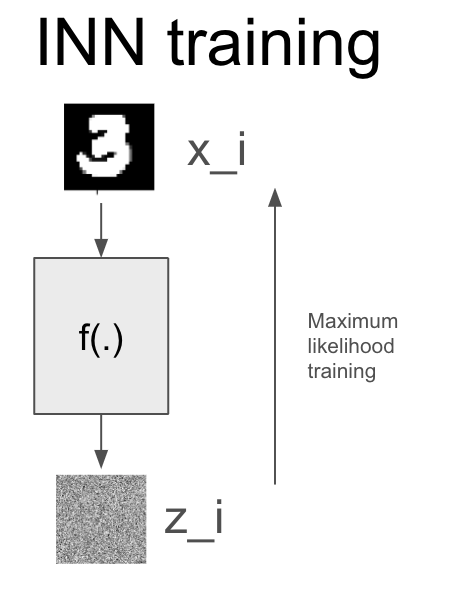
\includegraphics[width=0.30\columnwidth]{fig_datasynth/inn_train.png}  
            
    \vspace{-2pt}
    \caption{\label{tab:feat_extr_results_randinit} This will be a table... feature evaluation with randomly initialized weights.}
    \vskip -0.0in 
\end{figure}

        
\begin{figure}
    \vskip -0.2in 
    \centering

    % \includegraphics[width=0.80\columnwidth]{Images/feat_eval_pretrained.png} 
    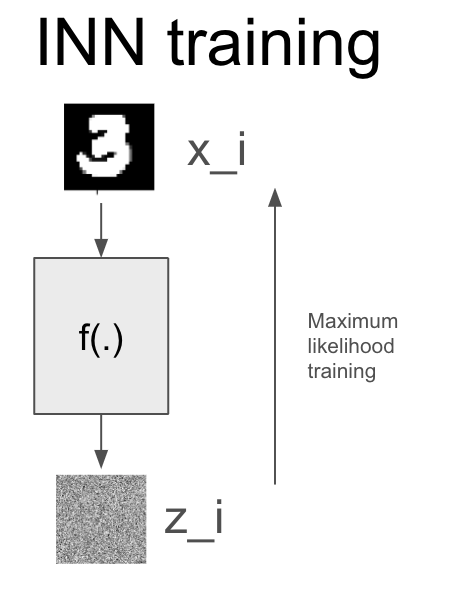
\includegraphics[width=0.30\columnwidth]{fig_datasynth/inn_train.png}  
            
    \vspace{-2pt}
    \caption{\label{tab:feat_extr_results_pretrained}  This will be a table... feature evaluation with pre-trained weights.}
    \vskip -0.0in 
\end{figure}

\begin{figure}
    \vskip -0.2in 
    \centering

    % \includegraphics[width=0.80\columnwidth]{Images/retrieval_eval_pretrained_RN50.png} 
    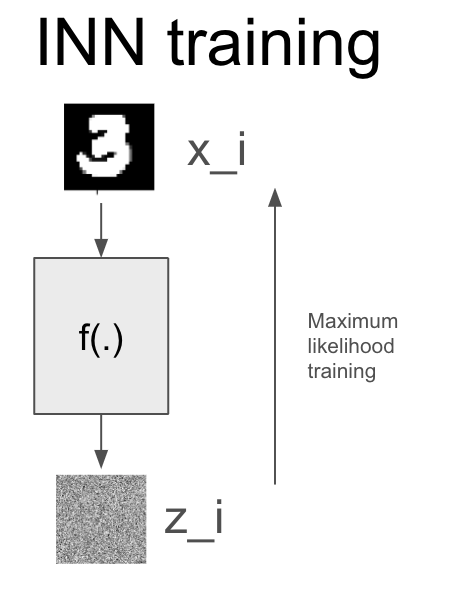
\includegraphics[width=0.30\columnwidth]{fig_datasynth/inn_train.png}  
            
    \vspace{-2pt}
    \caption{\label{fig:exp_feat_extr_retrieval_pretrained} Image (still to fix and make it look nice) of retrieval evaluation with pre-trained weights - RN50 model.}
    \vskip -0.0in 
\end{figure}
        

\begin{figure}
    \vskip -0.2in 
    \centering

    % \includegraphics[width=0.80\columnwidth]{Images/retrieval_eval_randinit_RN50.png} 
    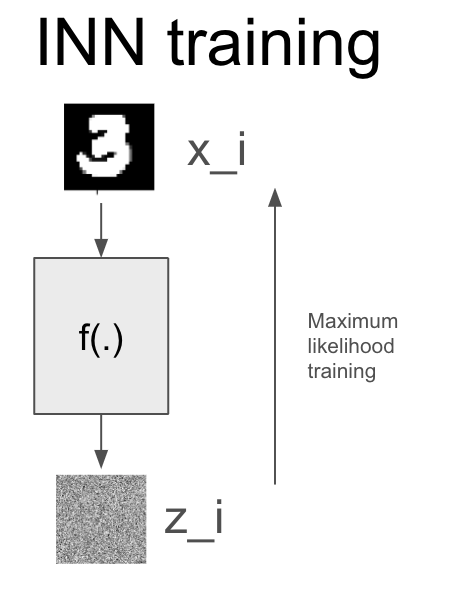
\includegraphics[width=0.30\columnwidth]{fig_datasynth/inn_train.png}  
            
    \vspace{-2pt}
    \caption{\label{fig:exp_feat_extr_retrieval_randInit} Image (still to fix and make it look nice) of retrieval evaluation with randomly initilised weights - RN50 model.}
    \vskip -0.0in 
\end{figure}

%%%%%%%%%%%%%%%% VRAE and clustering %%%%%%%%%%%%%%%%
\subsection{VRAE clustering for time series data.}
\label{subsec:2.3_featext_tech2}

This section describes the approach used to expand the feature extraction capabilities of MANOLO to the time series domain: variational auto-encoders (VAEs). These are a valuable alternative to extract features in applications where labeled data are scarce, pre-trained models are not available, or the target task is very specific and knowledge transfer is not effective. Concretely, we use the variational recurrent auto encoder (VRAE) proposed by Fabius and Amersfoort~\cite{2015_ICLRw_VRAE}. 

Subsection~\ref{subsubsec:VRAE_Meth} briefly introduces the VRAE model as a VAE, explainings its value as a feature extractor to be included in the MANOLO Data module, and provides details on the experimental setup used and the evaluation process followed to obtain the results reported in Subsection~\ref{subsubsec:VRAE_Res}. As this section is focused on time series, it will also focus on a common challenge in this modality: data class imbalance. We identified this challenge and report its effect in the results section. Section XXX includes the class imbalance in data as a challenge to be addressed for future iterations of the report. 
    
\subsubsection{Methodology}\label{subsubsec:VRAE_Meth}
VRAEs were originally designed for unsupervised time series clustering, providing discriminative and representative features, which according to the original publication is also a competitive approach to initialise recurrent neural networks (RNNs).
        
The VRAE is a model that combines Recurrent NNs with the variational auto-encoder architecture: an encoder block maps samples to a latent space, and a decoder block maps vectors from the latent space back to the sample space. VRAEs also applie the basic principle behind VAEs by producing an output tensor that resembles the input sample while passing through a Gaussian latent space of reduced dimensionality. This forced compression of the representations guides VAEs to learn a mapping function, the encoder, to a latent space that preserves relevant features and represents the distribution of the input data. Note that, simultaneously, the VRAE learns a mapping function, the decoder, that reconstructs an input sample given a vector in the latent space.

\paragraph{Feature evaluation setup.}  
To repurpose VRAEs for the MANOLO feature extraction functionality, we leverage the latent space learned by the VRAE and use the latent vectors as extracted features. In this setup, the trained encoder of the VRAE becomes the feature extractor model. The evaluation of these features is carried out following the procedure described in Section~\ref{subsubsec:NNfeatExtr_Meth}, i.e. we report accuracy with a linear classifier, with a non-linear classifier, and with a KNN-classifier. In addition, due to the class imbalance in the datasets studied in this section, we report the balanced accuracy metric, as implemented in the scikit-learn library~\cite{scikit-learn}, for these three classifiers~\footnote{\url{https://scikit-learn.org/stable/modules/generated/sklearn.metrics.balanced_accuracy_score.html}}. This metric reports a more accurate measure of the performance of a model when the number of samples in each class is imbalanced.  
    
\paragraph{Experimental setup.} 
The VRAE implementation integrated in MANOLO closely follows the architecture and adopts most of the hyperparameters suggested in the original paper~\cite{2015_ICLRw_VRAE}. Hence, the features extracted are vectors of 20 dimensions. To accommodate the selected datasets, however, we increased the number of layers to two and selected a learning rate of 0.0005. We use four time series datasets easily accessible from the tslearn library~\cite{JMLR:v21:20-091}: ECG5000, ElectricDevices, FordA, and FordB. For all the datasets we used the same pre-processing: min-max normalised all the samples and rounded all the values to two decimals. We followed the train-validation split defined in the tslearn library and used the train set to train the VRAE and the classifiers for the evaluation, then computed the reported metrics on the validation set.

The Ecg5000 dataset~\cite{2000_physiobank_ECG5000} is constituted by 5000 randomly selected heart bits from a patient with severe congestive heart failure automatically annotated as one of five classes. The distribution of samples is heavily biased towards the first and second class, which have over 4000 samples between them while the third, fourth, and fifth classes have less than 500 samples altogether. This dataset is often used in medical time series research for anomaly detection and classification tasks~\cite{2015_ACM_ecg5000InitialPaper, 2022_IEEE_tsmae, 2022_IEEE_lightweight}, where the 5000 samples are usually split into 4500 samples for testing and 500 for training. The imbalance of the data labels makes it a challenging dataset well-suited to one of the purposes of MANOLO: address possible biases. Each sample has a length of 140 measurements and a single dimension. 

The ElectricDevices dataset, availale in the UCR time series archive~\cite{2019_IEEE_ucr}, is a collection of electricity consumption readings from 251 households sampled in two-minute intervals over a month, resulting in 16637 samples split into 8926 samples for the train set and 7711 for the test set. The samples are annotated into one of seven classes. In this case, five of the classes have around 1000 samples each while the other two around 2000 each. This illustrates a less severe type of class imbalance when compared to the ECG5000 dataset. ElectricDevices is a single variable dataset and the length of each sample is xxx measurements. The ElectricDevices dataset is commonly used in time series classification, forecasting, and explainability among others~\cite{2023_Springer_TSandXAI, 2024_IEEE_gmtpm, 2020_IEEE_fastee, 2016_SEKE_time}.

Finally, the FordA and FordB datasets, also from the UCR archive~\cite{2019_IEEE_ucr} are a collection of samples from an automobile subsystem labeled to identify the presence of a particular symptom resulting in a binary classification task. The first dataset is split into a set of 3601 samples for training and 1320 for testing, and the second dataset into 3636 and and 810 for training and testing respectively. All the samples consist of 500 measurements from a single sensor. Additionally, FordB dataset presents a more challenging task than FordA due to the inclusion of noise in the measurements in the test set. These datasets are used in time series research as benchmarks for binary tasks as well as robustness against noisy measurements~\cite{2021_ICML_voice2series, 2022_arxiv_hypertime, 2023_Springer_deep}.

    *** 
            
\subsubsection{Results}\label{subsubsec:VRAE_Res}

We have evaluated the latent space learned by the VRAE both qualitatively and quantitatively. The former consist of the standard evaluation used for self-supervised representation learning, described in Section XXX. In this case we use the encoder of the trained VRAE as a feature extractor and represent each input sample as a vector from the latent space. The latter consist of a PCA and tSNE visualization of the latent space that illustrates the ability of the encoder to allocate samples from a given class in a particular region of the space, allowing for a more efficient clustering of the samples.

Table~\ref{fig:exp_vrae_1} shows the results of a linear classifier, a KNN classifier and a non-linear classifier trained on the features from the train set extracted with the encoder of the VRAE, i.e. vectors from the latent space, and evaluated on the test set with the available labels. Table~\ref{fig:exp_vrae_2} reports the performance of the same evaluations under the balanced accuracy metric. .... This provides an accurate indication of the ability of the VRAE to extract discriminative features in terms of sample class. XXXX. ==> \textbf{\textit{Re-running some of the models, FordA and FordB performance is the same as taking random chance.}}

\begin{figure}
    \vskip -0.2in 
    \centering
    % \includegraphics[width=0.80\columnwidth]{Images/vrae_eval_acc.png}    
    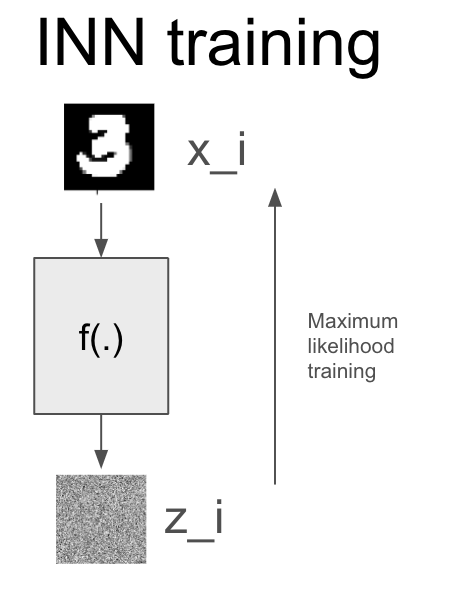
\includegraphics[width=0.30\columnwidth]{fig_datasynth/inn_train.png}    
    \vspace{-2pt}
    \caption{\label{fig:exp_vrae_1} Make a table out of this.}
    \vskip -0.0in 
\end{figure}
        
\begin{figure}
    \vskip -0.2in 
    \centering
    % \includegraphics[width=0.80\columnwidth]{Images/vrae_eval_acc.png}    
    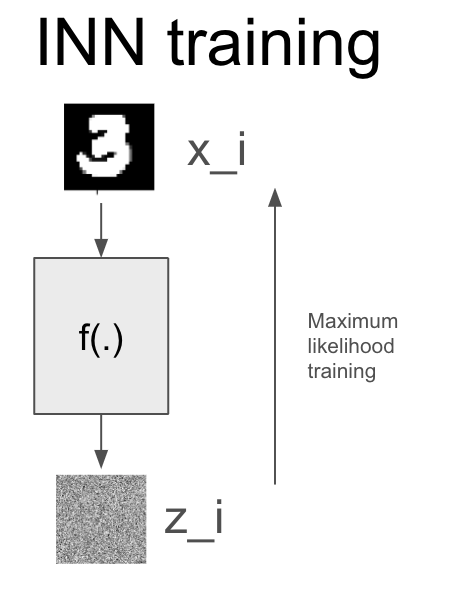
\includegraphics[width=0.30\columnwidth]{fig_datasynth/inn_train.png}      
    \vspace{-2pt}
    \caption{\label{fig:exp_vrae_2} Make a table out of this.}
    \vskip -0.0in 
\end{figure}

        
Figure xx provide several illustrations of the embedded space and its ability to separate features. The image show how some of the classes fall in nearby regions of the space. In particular... xxx. It is worth noting that this is only a visualization method and not a quantitative, reliable manner to evaluate the performance of a classifier. The techniques used (PCA and tSNE) project the features in two-dimensional plots and this remove nuances and details present in the original features in higher dimensional spaces.



\begin{figure}
    \vskip -0.2in 
    \centering
    % \includegraphics[width=0.80\columnwidth]{Images/vrae_eval_acc.png}    
    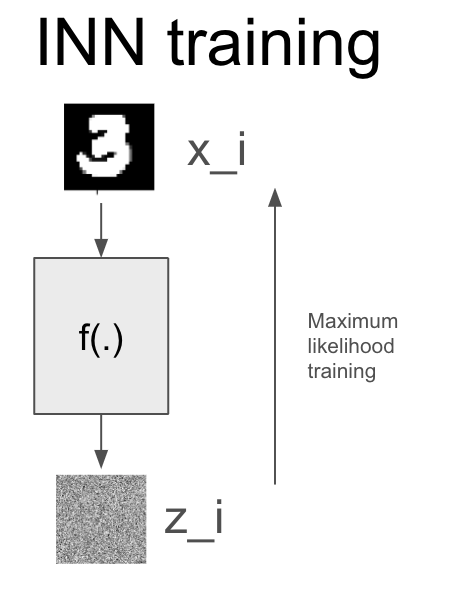
\includegraphics[width=0.30\columnwidth]{fig_datasynth/inn_train.png}  
    \vspace{-2pt}
    \caption{\label{fig:exp_vrae_3} Visualisation from left to right: ECG5000, ElectricDevices, FordA, and FordB. Top PCA and bottom tSNE.}
    \vskip -0.0in 
\end{figure}
   
%%%%%%%%%%%%%%%% %%%%%%%%%%%%%%%% %%%%%%%%%%%%%%%%
%%%%%%%%%%%%%%%%   Conclusion   %%%%%%%%%%%%%%%%
%%%%%%%%%%%%%%%% %%%%%%%%%%%%%%%% %%%%%%%%%%%%%%%%
\section{Conclusion}
\label{sec:conclusion}